\chapter{LITERATURE REVIEW}

\section{Human papillomavirus and cervical cancer}

\subsection{Epidemiology of cervical cancer}

Cervical cancer is the fourth most frequently diagnosed malignancy and the fourth leading cause of cancer death among women globally. According to GLOBOCAN 2020 estimates, approximately 604,000 new cases and 342,000 deaths were attributed to cervical cancer worldwide, with the vast majority of this burden concentrated in sub-Saharan Africa, South-East Asia, and Latin America \cite{sung2021}. In Vietnam, cervical cancer ranks among the top five cancers in women, with an estimated age-standardized incidence rate of 7.1 per 100,000 women-years and approximately 4,100 new cases diagnosed annually \cite{globocan2020vn}.

The striking geographic disparity in cervical cancer burden reflects fundamental inequities in access to primary prevention through HPV vaccination, secondary prevention through screening, and tertiary care through timely treatment of precancerous and cancerous lesions \cite{arbyn2020}. In high-income countries where organized screening programs have been established for decades, cervical cancer incidence has declined by 50--70\%; by contrast, many LMICs continue to experience rising trends \cite{bray2018}.

\subsection{HPV virology and natural history}

Human papillomavirus (HPV) is a small, non-enveloped, double-stranded DNA virus belonging to the \textit{Papillomaviridae} family. Over 200 HPV genotypes have been identified, of which approximately 40 infect the anogenital mucosa. These are classified as either low-risk (e.g., HPV 6, 11) or high-risk (e.g., HPV 16, 18, 31, 33, 45, 52, 58) based on their oncogenic potential \cite{doorbar2012}. HPV types 16 and 18 alone account for approximately 70\% of all cervical cancer cases globally \cite{delemore2017}.

The natural history of HPV-related cervical carcinogenesis follows a well-characterized multi-step pathway: initial HPV infection of the cervical transformation zone, viral persistence, progression through cervical intraepithelial neoplasia grades 1--3 (CIN1--CIN3), and ultimately invasive carcinoma. While most HPV infections are transient and resolve within 12--24 months through effective immune clearance, persistent infection with high-risk genotypes---particularly in the setting of immunosuppression or co-infections---can drive neoplastic transformation over a period of 10--20 years \cite{schiffman2016}.

\begin{figure}[htbp]
\centering
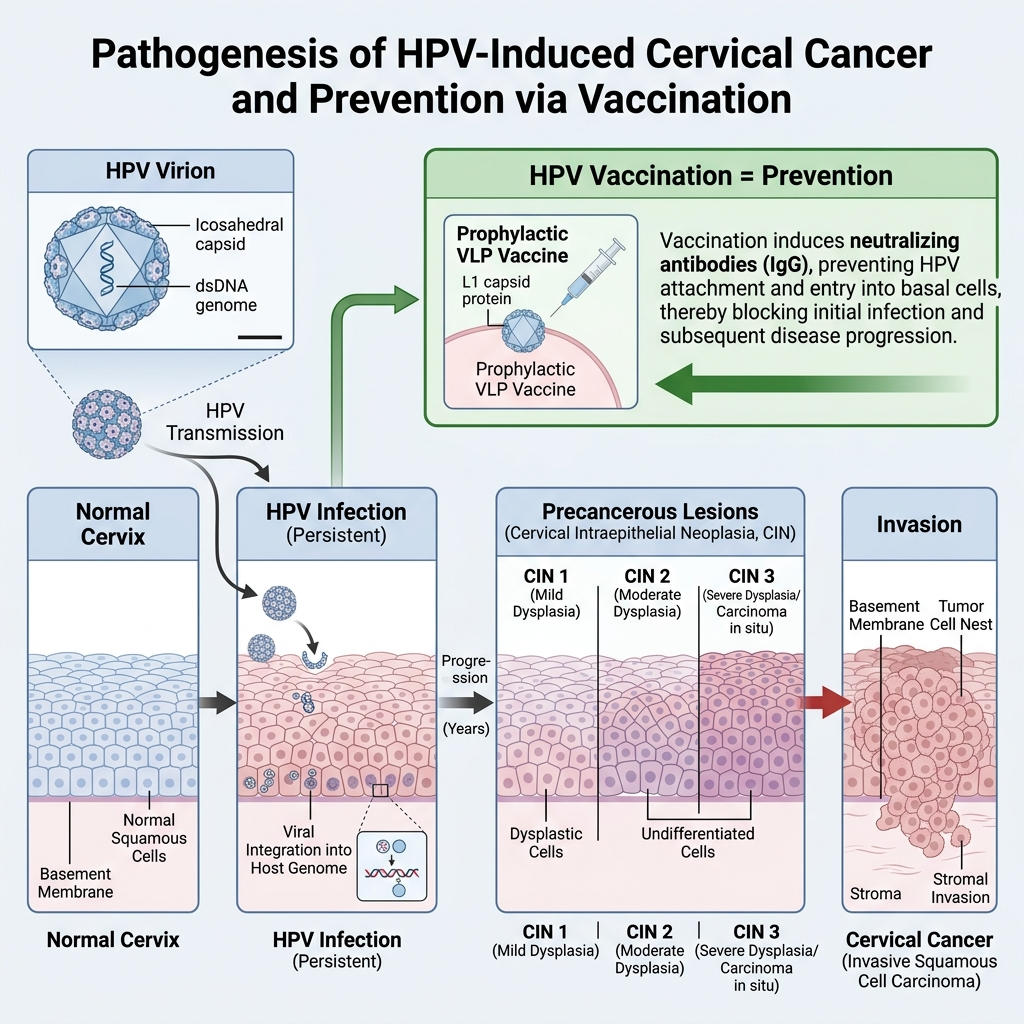
\includegraphics[width=0.85\textwidth]{Figures/hpv_cervical_cancer.png}
\caption{Natural history of HPV infection and cervical cancer development. HPV vaccination provides primary prevention by blocking initial infection, while screening programs enable secondary prevention through early detection and treatment of precancerous lesions.}
\label{fig:hpv_natural_history}
\end{figure}

\subsection{HPV vaccines: types and efficacy}

Three prophylactic HPV vaccines have been licensed and are currently available worldwide:

\begin{itemize}
	\item \textbf{Bivalent vaccine (Cervarix\textsuperscript{\textregistered})}: targets HPV types 16 and 18.
	\item \textbf{Quadrivalent vaccine (Gardasil\textsuperscript{\textregistered})}: targets HPV types 6, 11, 16, and 18.
	\item \textbf{Nonavalent vaccine (Gardasil 9\textsuperscript{\textregistered})}: targets HPV types 6, 11, 16, 18, 31, 33, 45, 52, and 58, potentially preventing up to 90\% of cervical cancers.
\end{itemize}

Large-scale randomized controlled trials and post-licensure surveillance data have demonstrated vaccine efficacy exceeding 90\% against persistent infection and precancerous lesions caused by vaccine-targeted HPV types when administered prior to HPV exposure \cite{lei2020,drolet2019}. The WHO currently recommends a one- or two-dose schedule for girls aged 9--14 years as the primary target population, with catch-up vaccination for females aged 15--26 \cite{who2022}.

Population-level impact has been substantial in countries with high vaccine coverage. A 2019 meta-analysis of data from 60 million individuals across 14 high-income countries demonstrated significant reductions in HPV 16/18 infections (83\% among girls aged 13--19), anogenital warts (67\%), and CIN2+ lesions (51\%) within 5--8 years of vaccine introduction \cite{drolet2019}.

\section{HPV vaccination globally and in Vietnam}

\subsection{Global vaccination landscape}

As of 2023, over 140 countries had introduced HPV vaccination into their national immunization programs. However, global coverage remains uneven: while many high-income countries have achieved coverage rates exceeding 70\%, coverage in LMICs---where the disease burden is greatest---remains below 15\% \cite{bruni2023}. The COVID-19 pandemic further disrupted vaccination programs, leading to an estimated 3.5 million missed doses worldwide between 2020 and 2022 \cite{who2023disruption}.

The persistent gap between vaccine availability and actual uptake in LMICs reflects a complex interplay of supply-side factors (cost, cold-chain logistics, health system capacity) and demand-side barriers (awareness, cultural beliefs, misinformation, distance to health facilities) \cite{gallagher2018}.

\subsection{HPV vaccination in Vietnam}

Vietnam's engagement with HPV vaccination began with a GAVI-supported demonstration project in 2006, initially targeting girls aged 11--12 years in selected provinces. The program was subsequently expanded through the national Expanded Programme on Immunization (EPI), although nationwide roll-out has proceeded gradually due to logistical and financial constraints \cite{nguyen2021}.

As of 2023, HPV vaccination in Vietnam remains partially dependent on out-of-pocket payment in many provinces, which disproportionately disadvantages women from lower socioeconomic backgrounds. The estimated national coverage among age-eligible females remains below 30\%, with marked urban--rural and inter-provincial disparities \cite{lamontagne2020,tran2022}. These patterns underscore the need for equity-focused analyses to inform targeted intervention strategies.

\section{Socioeconomic inequality in health: concepts and measurement}

\subsection{Defining health inequality}

Health inequality refers to systematic, avoidable, and unjust differences in health outcomes or determinants across population groups defined by social, economic, demographic, or geographic characteristics \cite{whitehead1991}. When these differences arise from modifiable socioeconomic circumstances rather than biological variation, they are termed health \textit{inequities} and carry a distinct normative imperative for policy action \cite{braveman2006}.

In the context of HPV vaccination, socioeconomic inequality manifests as differential awareness of and access to vaccination services across wealth strata. Such inequality is particularly concerning because it amplifies existing disparities: women who are poorest and least educated---and who often face the highest cervical cancer risk due to limited screening access---are also the least likely to be reached by vaccination programs \cite{paul2020}.

\subsection{The concentration index}

The concentration index (CI) is the most widely used summary measure of socioeconomic inequality in health. Formally, the CI is defined as twice the area between the concentration curve and the 45-degree line of equality \cite{wagstaff2000}:

\begin{equation}
CI = \frac{2}{\mu} \mathrm{cov}(y_i,\, r_i)
\label{eq:ci}
\end{equation}

\noindent where $y_i$ is the health variable for individual $i$, $r_i$ is the fractional rank of individual $i$ in the socioeconomic distribution, and $\mu$ is the population mean of $y$.

The CI ranges from $-1$ to $+1$. A positive value indicates that the health variable is concentrated among the wealthier (pro-rich inequality), a negative value indicates concentration among the poorer (pro-poor inequality), and zero implies perfect equality.

\subsection{The Erreygers correction and decomposition}

For bounded health variables (such as binary indicators of vaccination status), the standard CI may yield misleading comparisons across populations with different means. Erreygers (2009) proposed a corrected concentration index that satisfies mirror, level independence, and cardinal invariance properties \cite{erreygers2009}:

\begin{equation}
E(y) = \frac{4\mu}{b-a} \cdot CI
\label{eq:erreygers}
\end{equation}

\noindent where $a$ and $b$ are the lower and upper bounds of the health variable (0 and 1 for binary outcomes).

The Erreygers-corrected CI can be decomposed into the contributions of individual determinants using the relationship:

\begin{equation}
E(y) = 4 \sum_k \beta_k \bar{x}_k \cdot CI_k + \text{residual}
\label{eq:decomposition}
\end{equation}

\noindent where $\beta_k$ is the marginal effect of covariate $x_k$ from a probit model, $\bar{x}_k$ is the covariate mean, and $CI_k$ is the concentration index of the covariate with respect to socioeconomic rank. This decomposition enables researchers to quantify the percentage contribution of each factor---such as education, wealth, or geographic location---to the total observed inequality \cite{wagstaff2003,hosseinpoor2012}.

\section{Evidence on determinants of HPV awareness and vaccination}

A growing body of literature has examined factors associated with HPV vaccine awareness and uptake in LMIC settings. Key findings from systematic reviews and country-specific studies include:

\textbf{Socioeconomic status.} Higher household wealth is consistently associated with greater awareness and higher vaccination rates. Studies in sub-Saharan Africa, South-East Asia, and Latin America have documented wealth-related gradients of 2--5 fold in vaccination coverage \cite{paul2020,simo2020}.

\textbf{Education.} Women with secondary or higher education are significantly more likely to have heard of HPV vaccination and to have been vaccinated, reflecting both greater health literacy and enhanced access to information \cite{nguyen2021,bisi2022}.

\textbf{Urban--rural residence.} Urban women generally have higher awareness and vaccination rates, likely due to proximity to health facilities, greater media exposure, and higher density of vaccination service points \cite{tran2022,gallagher2018}.

\textbf{Ethnicity.} In multi-ethnic societies, ethnic minority women often exhibit lower awareness and uptake, attributable to language barriers, cultural beliefs, geographic isolation, and systemic marginalization \cite{pham2020}.

\textbf{Mass media and ICT exposure.} Exposure to newspapers, radio, television, internet, and mobile communication has been positively associated with health knowledge and preventive behavior uptake in numerous health domains, including vaccination \cite{wakefield2010,laz2012}.

\textbf{Age and marital status.} Younger women and those who are unmarried may be more receptive to vaccination messages, though actual uptake patterns vary by country and program design \cite{bruni2023}.

\section{Research gap and rationale}

While the determinants of HPV vaccination have been extensively studied in high-income settings, several critical gaps remain in the Vietnamese context:

\begin{enumerate}
	\item \textbf{Lack of inequality-focused analysis.} Most Vietnamese studies report prevalence and associations but do not quantify the magnitude of socioeconomic inequality using standardized indices.
	\item \textbf{Limited decomposition evidence.} No nationally representative study has decomposed the sources of inequality in HPV awareness and vaccination in Vietnam using the Erreygers method.
	\item \textbf{Awareness--vaccination gap.} The phenomenon whereby women are aware of the vaccine but fail to receive it---the ``awareness--vaccination gap''---has received limited attention, yet it represents a distinct policy-relevant outcome.
	\item \textbf{Outdated data.} Previous Vietnamese studies relied on smaller regional samples or earlier survey rounds. The MICS6 dataset (2020--2021) provides the most recent nationally representative evidence available.
\end{enumerate}

\section{Conceptual framework}

Building on the social determinants of health framework (WHO Commission, 2008) and the behavioral model of health services utilization (Andersen, 1995), this study posits that HPV vaccine awareness and uptake are shaped by a constellation of predisposing, enabling, and reinforcing factors operating at the individual, household, and community levels.

\begin{figure}[htbp]
\centering
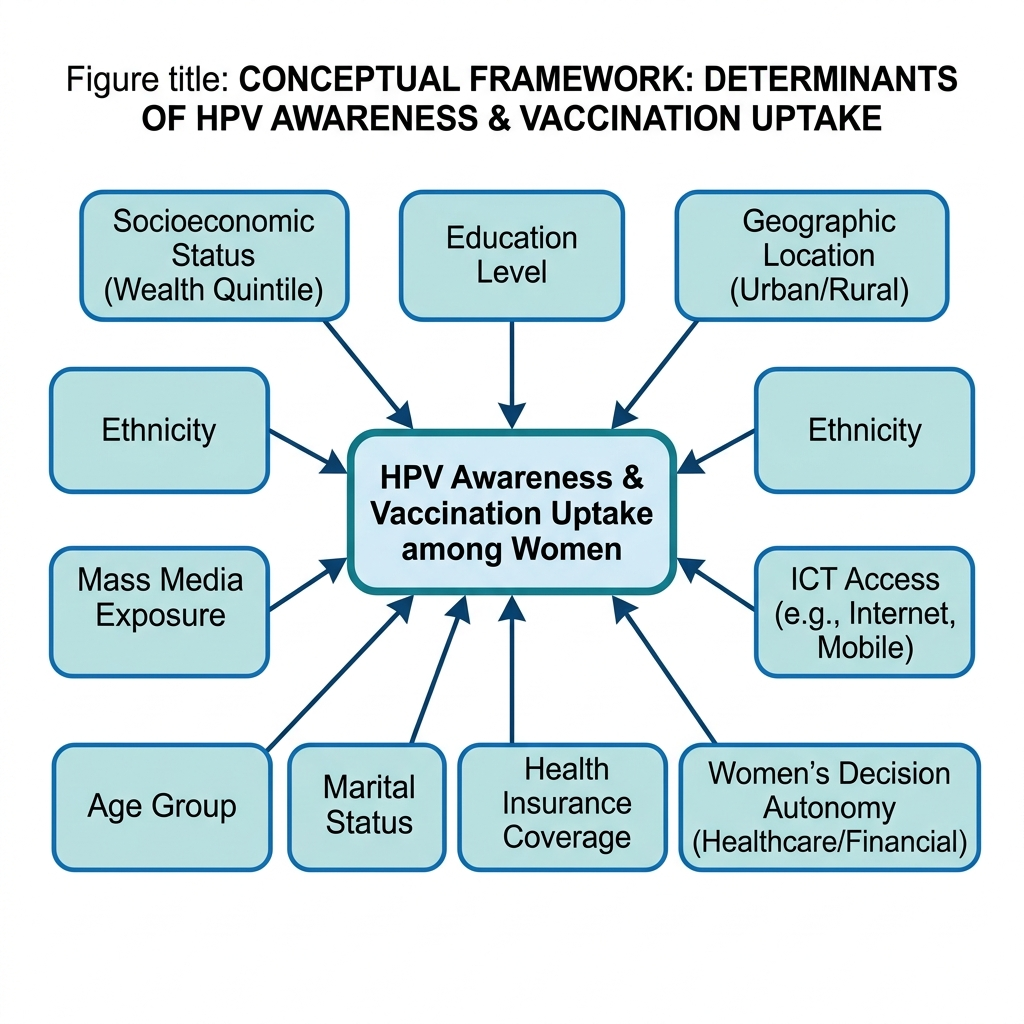
\includegraphics[width=0.88\textwidth]{Figures/conceptual_framework.png}
\caption{Conceptual framework illustrating the determinants of HPV vaccine awareness and vaccination among women aged 15--29 in Vietnam. Socioeconomic position, education, geographic location, ethnicity, and information exposure collectively shape both awareness and uptake, generating the observed inequality patterns.}
\label{fig:conceptual_framework}
\end{figure}

As depicted in Figure~\ref{fig:conceptual_framework}, the framework identifies the following key pathways:

\begin{itemize}
	\item \textbf{Structural determinants}: wealth quintile, education level, and urban/rural residence establish the fundamental socioeconomic gradient.
	\item \textbf{Intermediary determinants}: health insurance coverage, mass media and ICT exposure, and decision-making autonomy mediate the relationship between structural position and health behavior.
	\item \textbf{Individual characteristics}: age, marital status, sexual experience, and ethnicity modify vulnerability and exposure patterns.
\end{itemize}

This framework guides the selection of covariates for the multivariable Poisson regression and provides the theoretical basis for interpreting the Erreygers decomposition results presented in Chapter~3. 

Crucially, the framework conceptualizes the awareness--vaccination gap not merely as a sequential cognitive failure, but as a structural bottleneck where intermediary determinants exert differential pressures. While mass media and digital information exposure can successfully dismantle initial knowledge barriers, they are severely insufficient to overcome the profound financial and logistical hurdles of actual vaccine procurement in a predominantly privatized delivery system. This fundamental asymmetry dictates that the epidemiological predictors of awareness will diverge significantly from the predictors of final vaccine uptake.

Furthermore, the model acknowledges the intersectionality of these health determinants. For instance, ethnic minority status in Vietnam frequently intersects with geographic remoteness, language barriers, and lower baseline wealth, thereby compounding structural disadvantages at multiple levels of the health-seeking process. By mapping these interconnected pathways, the framework ensures that our subsequent econometric decomposition does not merely isolate abstract statistical associations. Instead, it precisely locates the actionable public health levers---whether universal health financing, targeted community outreach, or educational equity---required to dismantle the systemic inequities that sustain cervical cancer vulnerability among Vietnamese women.